% Entorno empresarial.
\chapter{Entorno Empresarial}

\vspace{5 mm}


	En el presente capítulo se exponen las características fundamentales de la empresa en la que fue realizado el proyecto. En la primera sección se explican los antecedentes o descripción histórica de la empresa. En la segunda, tercera y cuarta sección, se detallan su visión, misión y valores respectivamente. En la quinta seccion detalla la ubicación física de la empresa. La sexta sección explica la estructura organizacional de la empresa. Y finalmente, en la séptima sección se expone la ubicación del pasante dentro de dicha estructura empresarial.\cite{TDX}

\section{Antecedentes} \label{sect:Antecedentes}

	Tedexis, es una empresa regional pionera en soluciones móviles para compañías, especialmente en las áreas de banca y comercio móvil. Desde su fundación en el año 2000, ha alcanzado el liderazgo regional con el mayor número de implementaciones exitosas en el mercado,
convirtiendose en referencia no sólo en Latinoamérica, sino globalmente. 
\newline	
\newline
\indent Tedexis ofrece productos y servicios avanzados que son implementados 100\% por talento Venezolano, ayudando a crear un mundo donde las transacciones y el intercambio de información se realice a través de la tecnología adecuada al tiempo adecuado, desde cualquier parte.

\section{Misión} \label{sect:Mision}
	Exceder las expectativas de nuestros clientes mediante soluciones de tecnología móvil y talento humano comprometido e innovador.\cite{TDX}

\section{Visión} \label{sect:Vision}
	Ser una empresa centrada en el cliente, reconocida por su propuesta de valor superior en constante evolución, y por la competencia y motivación de su innovador capital humano.\cite{TDX}

\section{Valores}
\begin{itemize}[noitemsep,nolistsep]
\item Fans del servicio: e\textbf{X}ceder las expectativas del cliente.
\item Compromiso: cumplir lo que se ofrece y ofrecer \textbf{+} de lo que se espera.
\item Innovación: haz \textbf{+} piensa diferente \textbf{:)}.
\item Excelencia: la única manera de hacer las cosas.
\item Aprendizaje: ser \textbf{+} cada día.
\item Equipo\textbf{+}: orgullosos de ser \textbf{TEDEXIS x + :)}.
\end{itemize}

\section{Estructura Organizacional} \label{sect:Estructura Organizacional}
	En la Figura ~\ref{fig:estsyn} se presenta la estructura organizacional de la empresa, se tienen 5 áreas importantes entre las que se tienen:


\begin{itemize}[noitemsep,nolistsep]
\item \textbf{Dirección de comercialización y mercadeo}: es la encargada de la gestión de ventas y relación con los clientes actuales y prospespectos, promoviendo actividades que permitan desde su detección hasta el cierre de negociación.
\item \textbf{Dirección de producto}: encargada de la creación de productos en la organización. Son los responsables del desarrollo de software desde el inicio hasta su maduración y consolidación. En esta dirección fue ubicado el pasante durante todo el proyecto de pasantias.
\item \textbf{Dirección de operaciones}: dirección encargada del mantenimiento de los productos en producción de la empresa desde un enfoque técnico.
\item \textbf{Dirección de ingeniería de soluciones}: esta dirección es la encargada de gerenciar los nuevos y futuros proyectos dentro de la empresa. Generan prototipos de soluciones a problemas relevantes en los distintos departamentos.
\item \textbf{Dirección de planificación y seguimiento}: área encargada de velar por la calidad de los servicios que ofrece la empresa en forma global, desde procesos, metodologías de desarrollo, ejecución de proyectos y satisfacción de los clientes.
\end{itemize}

\begin{figure}[ht]
  \centering
  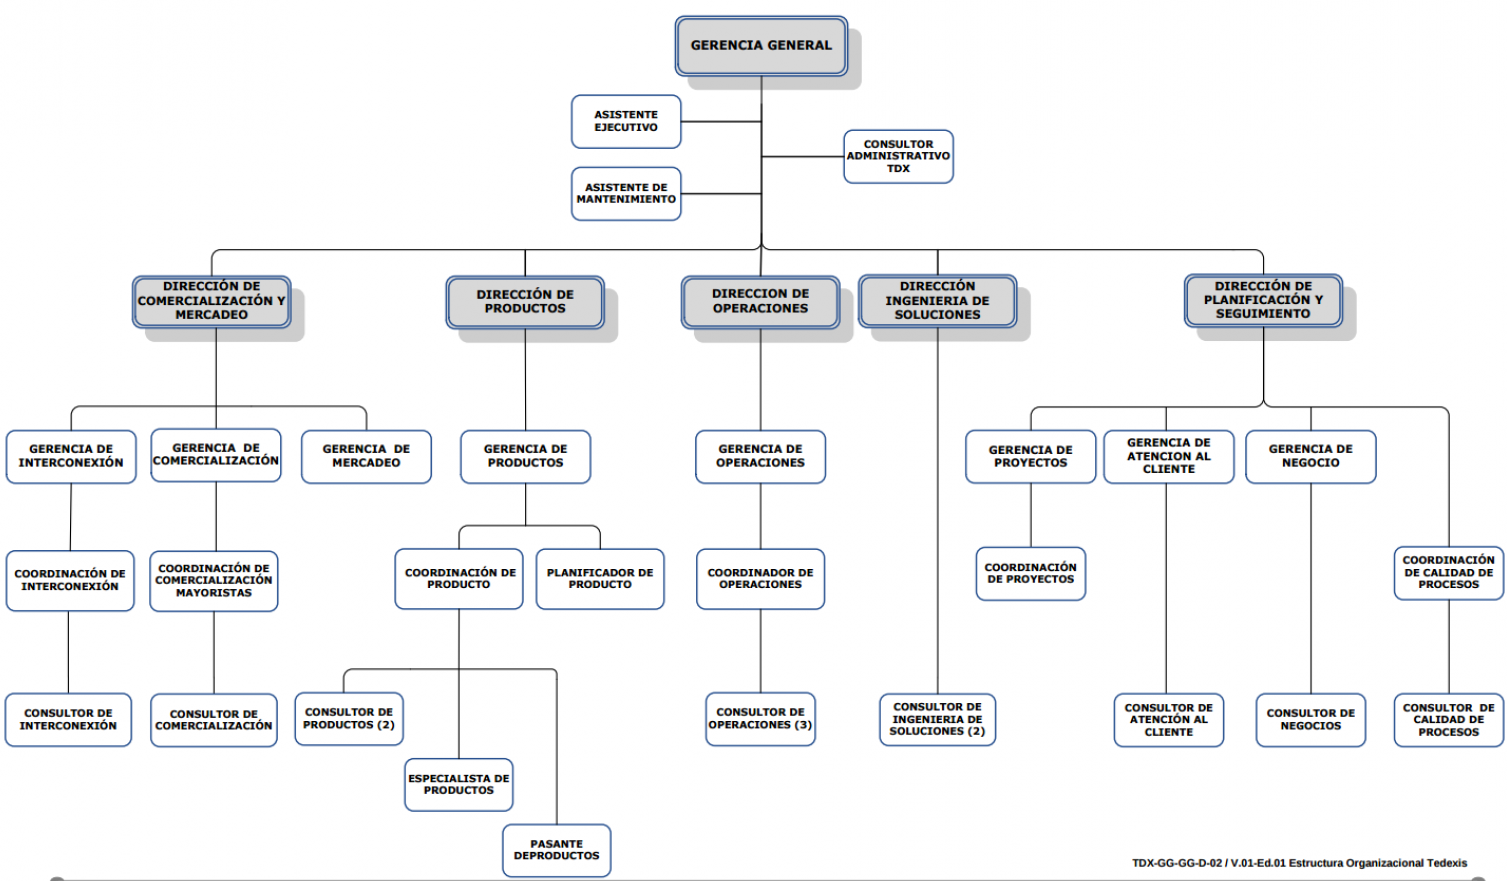
\includegraphics[scale=0.3,type=png,ext=.png,read=.png]{imagenes/organigrama} \\
  \caption{Estructura Organizacional de Tedexis}
  \label{fig:estsyn}
\end{figure}
